\documentclass[10pt,preprint2]{aastex}
\usepackage[a4paper,asymmetric,left=0.75in,right=0.75in,top=0.75in,bottom=0.75in]{geometry}
\AtBeginDocument{\newgeometry{asymmetric,left=0.75in,right=0.75in,top=0.75in,bottom=0.75in}\hoffset=0pt\setlength{\columnsep}{0.3in}\pagestyle{fancy}\fancyhf{}\fancyhead[L]{\small ASTRON 128 Astronomy Data Science Laboratory}\fancyhead[R]{\small Lab 3}\fancyfoot[C]{\thepage}}
\usepackage{amsmath, amsfonts, amssymb}
\usepackage{hyperref}
\usepackage{graphicx}
\usepackage{tikz}
\usepackage{booktabs}
\usepackage{fancyhdr}
\setlength{\headheight}{11pt}
\addtolength{\topmargin}{-0.16pt}
\usepackage{float}
\usepackage{stfloats}
\usepackage{pdflscape}
\usepackage{placeins}
\usepackage{pdfpages}\usetikzlibrary{arrows.meta,positioning,fit,calc,shapes.geometric}

\makeatletter\def\frontmatter@abstractheading{}\makeatother
\renewcommand{\abstractname}{}

% TikZ styles for pipeline flowchart
\tikzset{
  flowbox/.style={rectangle, rounded corners=4pt, draw=black, thick,
                  fill=blue!10, text width=3.0cm, align=center,
                  minimum height=0.8cm, font=\small},
  decisionbox/.style={diamond, draw=black, thick, fill=orange!15,
                      text width=2.2cm, align=center, aspect=1.5,
                      font=\footnotesize},
  outputbox/.style={rectangle, draw=black, thick, fill=green!15,
                    text width=2.5cm, align=center, minimum height=0.8cm,
                    font=\small},
  arrow/.style={-{Stealth[length=6pt]}, thick},
  % Architecture diagram styles
  inputlayer/.style={rectangle, rounded corners=2pt, draw=black, thick,
                     fill=gray!20, text width=2.7cm, align=center,
                     minimum height=0.55cm, font=\footnotesize},
  convlayer/.style={rectangle, rounded corners=2pt, draw=black, thick,
                    fill=blue!15, text width=2.7cm, align=center,
                    minimum height=0.55cm, font=\footnotesize},
  poollayer/.style={rectangle, rounded corners=2pt, draw=black, thick,
                    fill=cyan!15, text width=2.7cm, align=center,
                    minimum height=0.5cm, font=\footnotesize},
  resblock/.style={rectangle, rounded corners=2pt, draw=black, thick,
                   fill=violet!15, text width=2.7cm, align=center,
                   minimum height=0.55cm, font=\footnotesize},
  fclayer/.style={rectangle, rounded corners=2pt, draw=black, thick,
                  fill=orange!20, text width=2.7cm, align=center,
                  minimum height=0.55cm, font=\footnotesize},
  outlayer/.style={rectangle, rounded corners=2pt, draw=black, thick,
                   fill=green!20, text width=2.7cm, align=center,
                   minimum height=0.55cm, font=\footnotesize},
  archarrow/.style={-{Stealth[length=4pt]}, thick},
}

\begin{document}

\title{Galaxy Image Classification and the Galaxy Merger Rate}
\author{Jun Rui Ting \\ \today\vspace{-2.5\baselineskip}}

\begin{abstract}
We present a convolutional neural network (CNN) pipeline for morphological classification of galaxies from Sloan Digital Sky Survey (SDSS) images, using Galaxy Zoo 2 (GZ2) citizen-science labels as training data. Starting from 61{,}578 galaxy images with 37 continuous morphological labels (vote fractions in $[0,1]$), we center-crop and resize images to $96 \times 96$ pixels ($\sim$20$\times$ reduction in pixel count), split 80/20 into training (49{,}262) and validation (12{,}316) sets, and establish a mean-prediction baseline validation RMSE of 0.1639. We train two backbone architectures --- a 4-block custom CNN (32/64/128/256 channels with dropout) and an 18-layer ResNet adapted for small inputs and sigmoid output --- and apply two optimization techniques to each: \texttt{ReduceLROnPlateau} learning-rate scheduling and random $[0, 360^\circ)$ rotation augmentation exploiting the rotational invariance of galaxy morphology. The augmented ResNet with LR scheduling achieves the best validation RMSE of 0.0965, a $\sim$41\% improvement over the baseline. Per-label scatter plots reveal that top-level morphological features (smooth vs.\ disk) are predicted accurately, while rare sub-classifications (rings, mergers, lens/arcs) remain challenging due to sparse training examples. We apply the trained model to 79{,}975 test images and estimate a galaxy merger fraction of $\sim$4.3\%, comparing to the $z \approx 0$ merger rate from \citet{Lotz2011} and discussing complicating factors including the distinction between merger rate (Gyr$^{-1}$) and instantaneous merger fraction.

\vspace{2.5\baselineskip}
\end{abstract}

%%% ---------------------------------------------------------------
\section{Introduction}
\label{sec:intro}
%%% ---------------------------------------------------------------

Understanding galaxy morphology is fundamental to tracing the evolutionary history of galaxies across cosmic time \citep{Conselice2014}. The visual classification of galaxies into categories --- elliptical, spiral, irregular, merging --- dates back to Hubble's original tuning fork diagram, and modern large-scale surveys have extended this classification to hundreds of thousands of galaxies through citizen science projects such as Galaxy Zoo \citep{Lintott2008}. Galaxy Zoo 2 \citep{Willett2013} refined the classification scheme to 37 continuous labels organized in a hierarchical decision tree, enabling nuanced morphological descriptions including bar presence, spiral arm count, bulge prominence, and disturbed/merging features.

However, human classification does not scale to the billions of galaxies that will be observed by upcoming surveys (LSST, Euclid, Roman). Convolutional neural networks (CNNs) offer an automated alternative: given sufficient training data, a CNN can learn to extract morphological features directly from pixel data \citep{Krizhevsky2020}. In this work, we train CNNs on GZ2 labels to predict all 37 morphological classifications simultaneously, then apply the trained model to estimate the galaxy merger fraction at $z \approx 0$.

Figure~\ref{fig:pipeline} provides an overview of the analysis pipeline.

\begin{figure*}[t!]
  \centering
  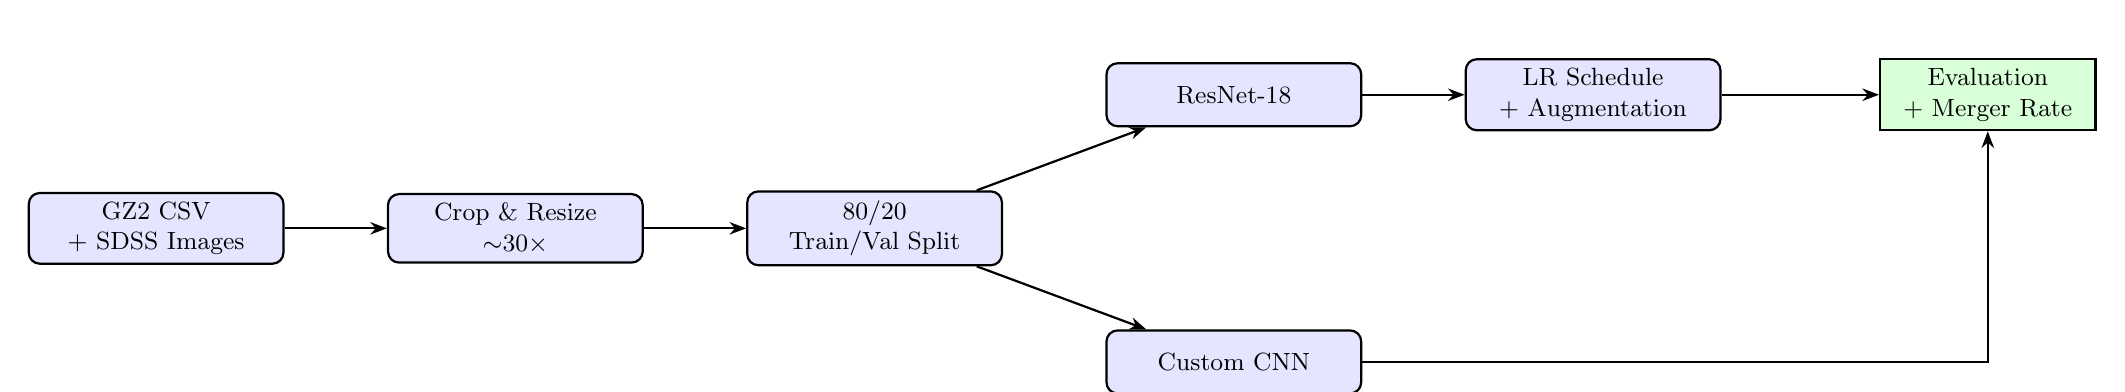
\begin{tikzpicture}[node distance=1.6cm and 1.3cm]
    \node[flowbox] (csv) {GZ2 CSV\\+ SDSS Images};
    \node[flowbox, right=of csv] (crop) {Crop \& Resize\\$\sim$30$\times$};
    \node[flowbox, right=of crop] (split) {80/20\\Train/Val Split};
    \node[flowbox, above right=0.8cm and 1.3cm of split] (resnet) {ResNet-18};
    \node[flowbox, below right=0.8cm and 1.3cm of split] (custom) {Custom CNN};
    \node[flowbox, right=of resnet] (opt) {LR Schedule\\+ Augmentation};
    \node[outputbox, right=2.0cm of opt] (eval) {Evaluation\\+ Merger Rate};
    \draw[arrow] (csv) -- (crop);
    \draw[arrow] (crop) -- (split);
    \draw[arrow] (split) -- (resnet);
    \draw[arrow] (split) -- (custom);
    \draw[arrow] (resnet) -- (opt);
    \draw[arrow] (custom.east) -| (eval.south);
    \draw[arrow] (opt) -- (eval);
  \end{tikzpicture}
  \caption{Analysis pipeline. SDSS galaxy images and GZ2 classification labels are preprocessed (crop, resize, split), then used to train a custom CNN and a ResNet-18. The best model is optimized with learning-rate scheduling and data augmentation, then evaluated on the validation and test sets. The final step estimates the galaxy merger fraction.}
  \label{fig:pipeline}
\end{figure*}

%%% ---------------------------------------------------------------
\section{Data Exploration}
\label{sec:data}
%%% ---------------------------------------------------------------

The training set consists of 61{,}578 SDSS $gri$-composite images ($424 \times 424$ pixels) and 37 GZ2 classification labels per galaxy. Each label is a vote fraction in $[0, 1]$ representing the proportion of human classifiers who assigned that morphological feature. The labels are organized hierarchically: top-level questions (smooth vs.\ disk vs.\ star/artifact) gate whether deeper questions (bar? spiral? arm count?) are asked.

\subsection{Label Distributions}

Figure~\ref{fig:label_distributions} shows normalized histograms of all 37 labels. Top-level labels (smooth, features/disk) exhibit broad, roughly bimodal distributions, while deeper labels (arm count, spiral tightness) are heavily concentrated near zero because most galaxies never reached those questions. This hierarchical concentration is a fundamental property of the GZ2 label space and presents a challenge for the CNN: the model must learn that most labels are near-zero for most galaxies.

\begin{figure}[H]
  \centering
  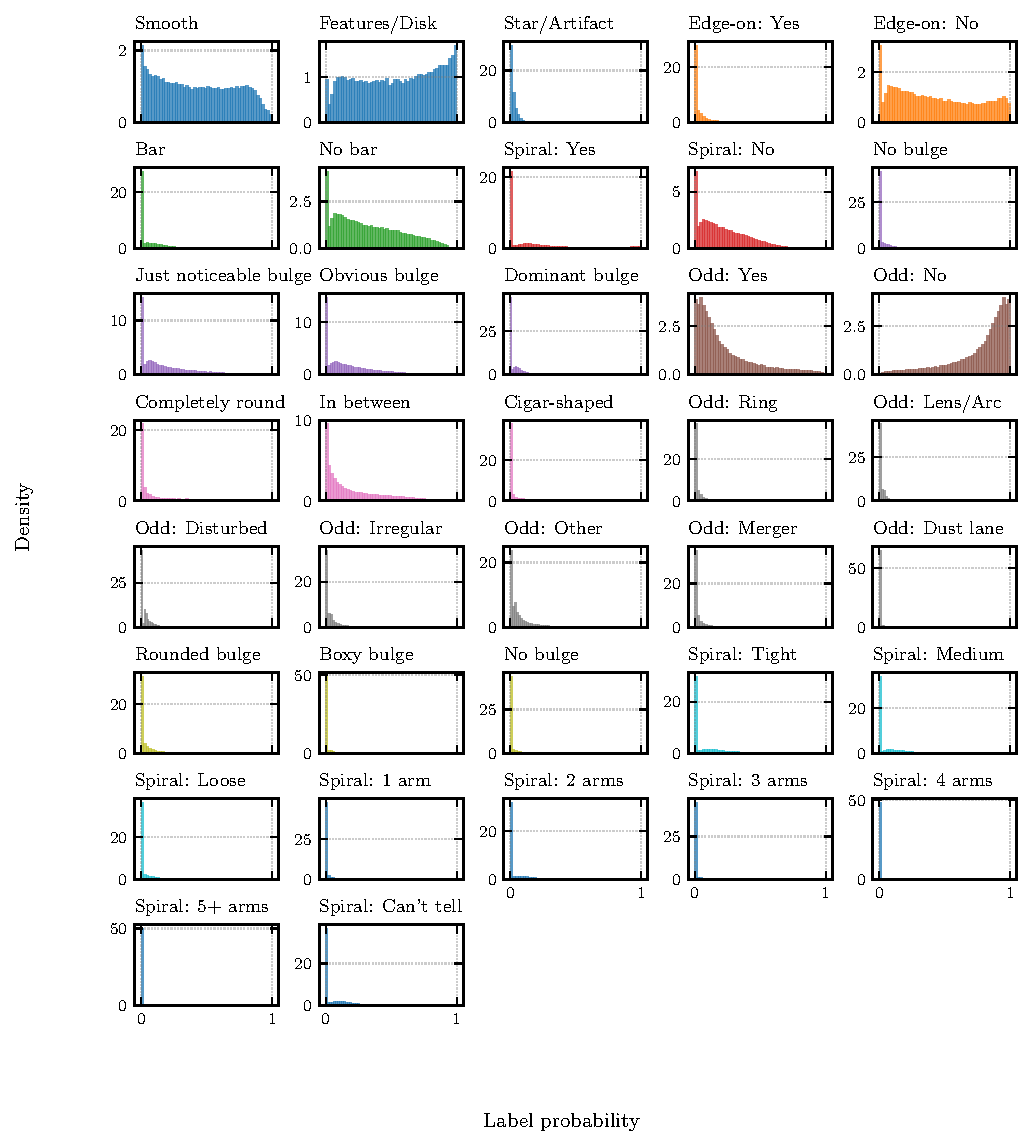
\includegraphics[width=\textwidth]{figures/fig_label_distributions.pdf}
  \caption{Normalized histograms of all 37 GZ2 classification labels. Top-level labels show broad distributions; deeper hierarchical labels are concentrated near zero.}
  \label{fig:label_distributions}
\end{figure}

\subsection{Prototype Images}

Figure~\ref{fig:prototype_images} shows the prototype image (highest vote fraction) for each label, providing a visual dictionary of the classification scheme.

\begin{figure}[H]
  \centering
  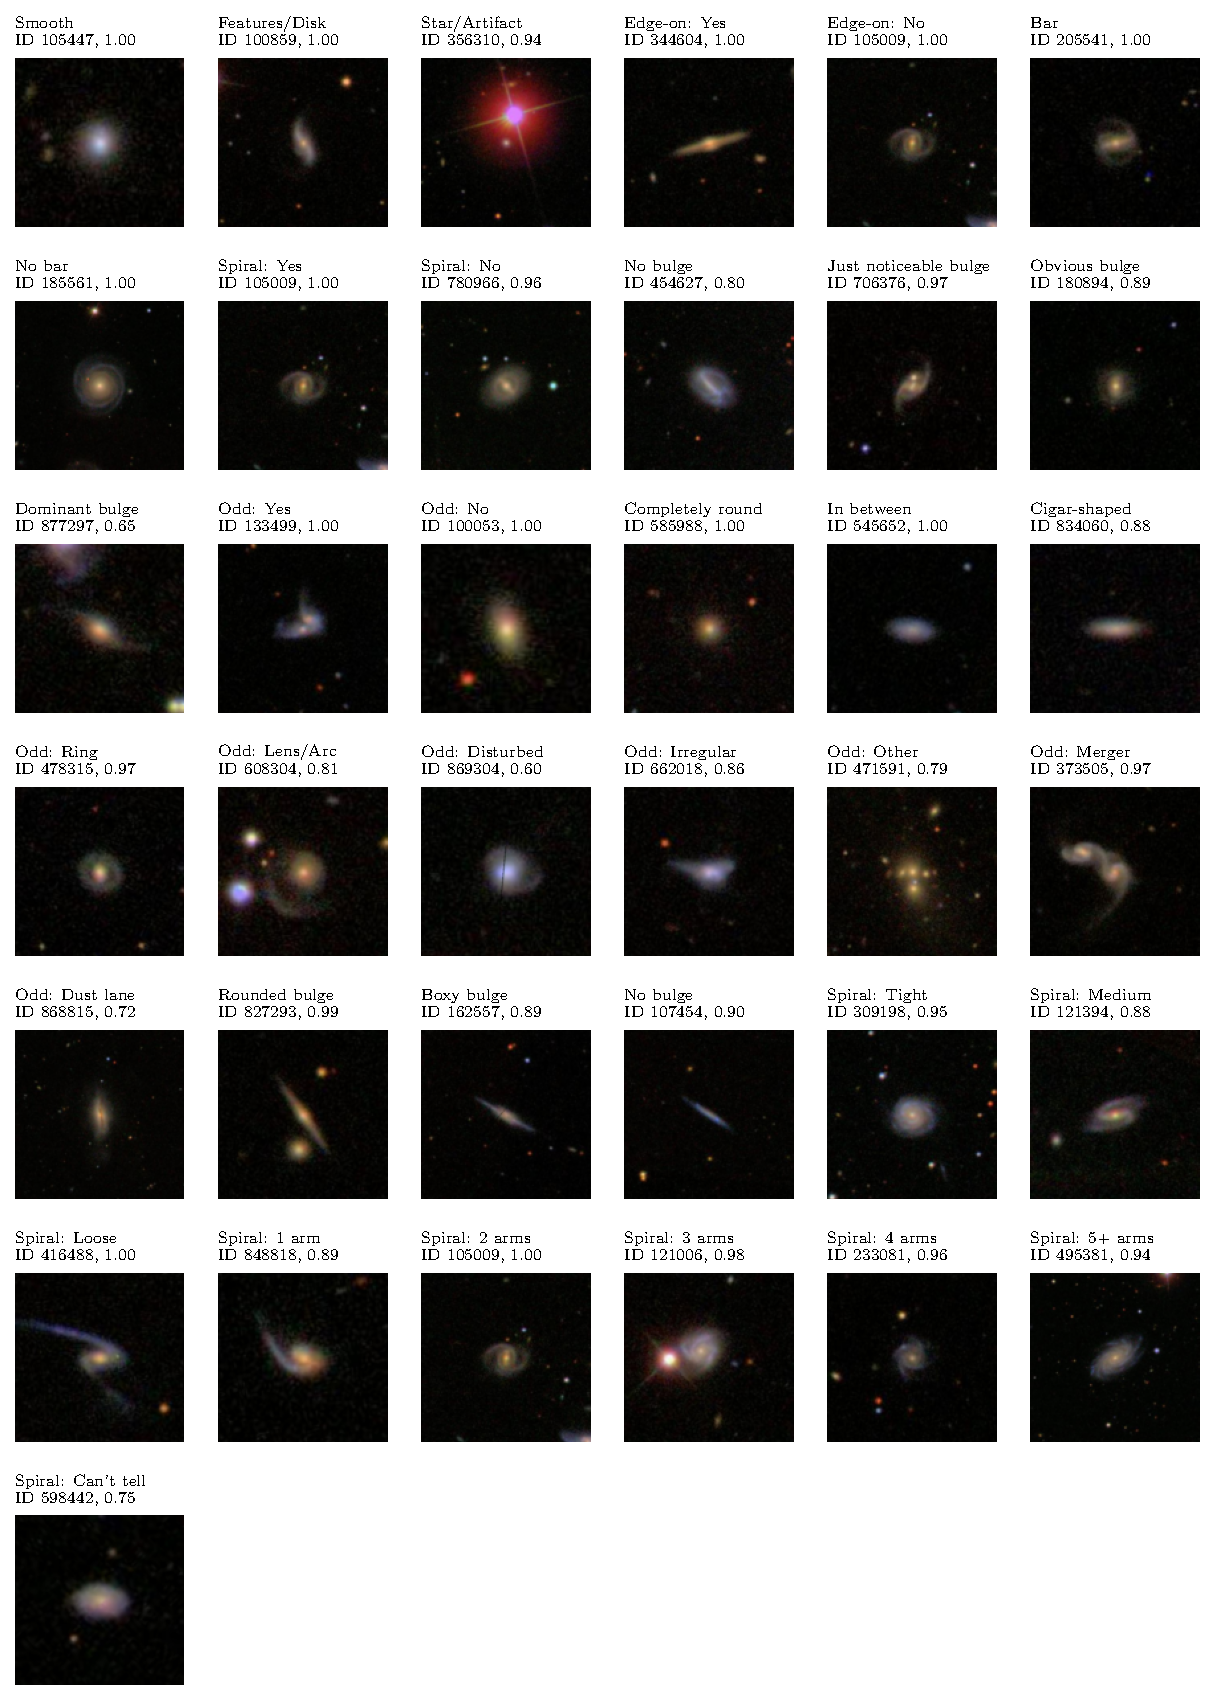
\includegraphics[width=\textwidth]{figures/fig_prototype_images.pdf}
  \caption{Prototype images: the galaxy with the highest vote fraction for each of the 37 labels.}
  \label{fig:prototype_images}
\end{figure}

\subsection{Label Correlations}

Figure~\ref{fig:correlation_matrix} shows the $37 \times 37$ Pearson correlation matrix. Strong negative correlations within each question confirm mutually exclusive categories, while positive correlations along the hierarchical tree reflect parent--child dependencies. The expected correlation for two mutually exclusive binary labels is $\rho = -1$; the observed values are close to this for Class1.1/1.2 and Class2.1/2.2.

\begin{figure}[H]
  \centering
  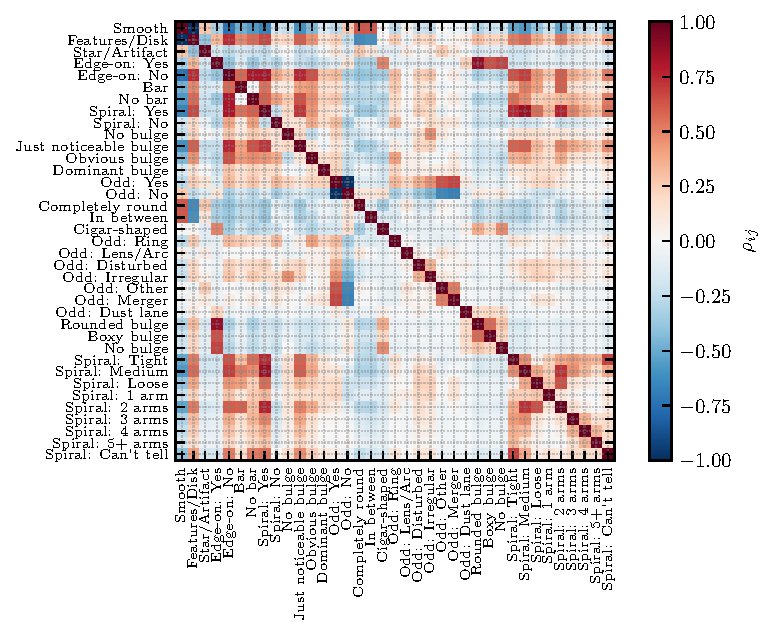
\includegraphics[width=\textwidth]{figures/fig_correlation_matrix.pdf}
  \caption{Pearson correlation matrix of all 37 labels. Block-diagonal structure reflects the hierarchical decision tree.}
  \label{fig:correlation_matrix}
\end{figure}

\subsection{Diagnostic Analyses}

To better understand the structure of the label space and the imbalance challenges facing the CNN, we perform several diagnostic analyses. Figure~\ref{fig:label_tree} visualizes the GZ2 hierarchical decision tree, making explicit which labels gate which downstream questions. Figure~\ref{fig:hierarchical_correlation} reorders the correlation matrix by tree branch, exposing block structure that the unordered matrix obscures. Figure~\ref{fig:label_tsne} shows a t-SNE embedding of the 37-dimensional label space; the manifold separates cleanly along the smooth/disk axis but rare classes form sparse, isolated clusters. Figure~\ref{fig:effective_sample_size} quantifies the effective sample size $N_{\rm eff} = (\sum f_i)^2 / \sum f_i^2$ per label, demonstrating that several deeper-tree labels have $N_{\rm eff} \lesssim 1000$, far below the nominal 61{,}578.

\begin{figure}[H]
  \centering
  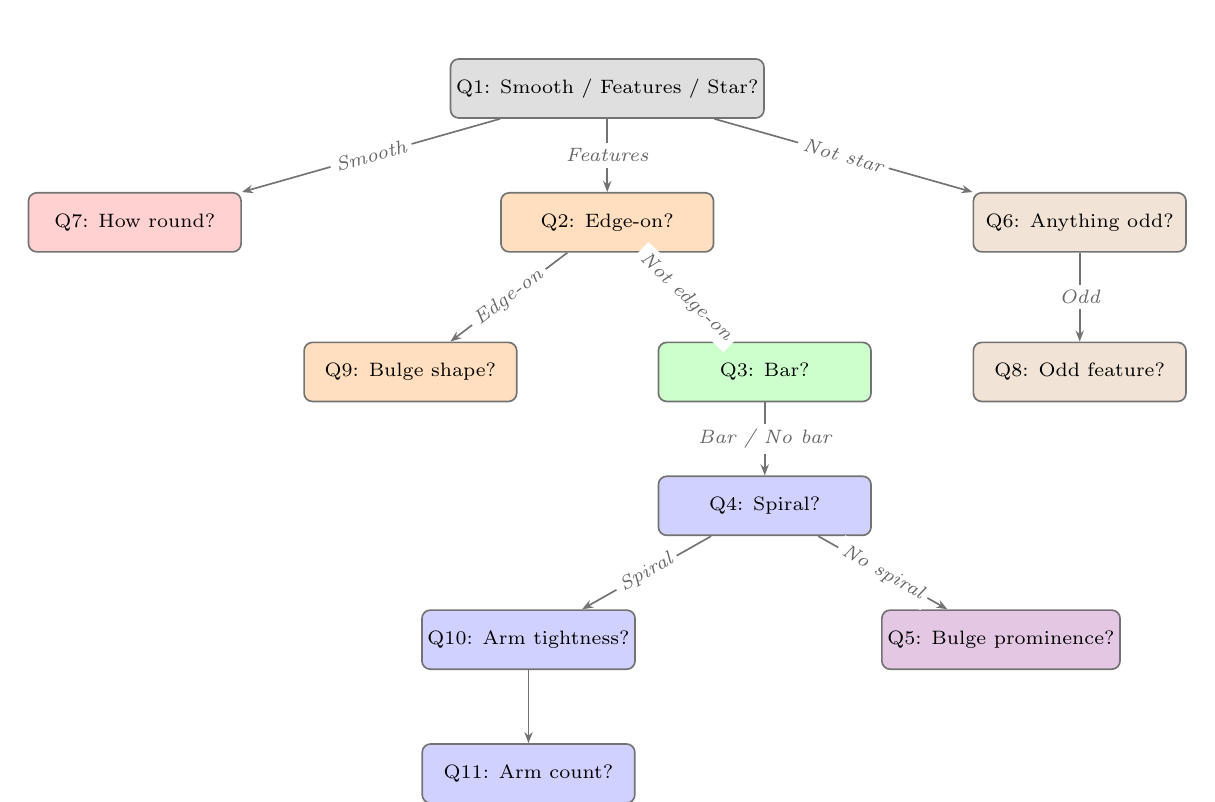
\begin{tikzpicture}[
      qbox/.style={rectangle, rounded corners=3pt, draw=black!55,
                   semithick, minimum width=2.7cm, minimum height=0.75cm,
                   align=center, font=\scriptsize, inner sep=2pt},
      qroot/.style={qbox, fill=gray!25},
      qsmooth/.style={qbox, fill=red!18},
      qedgeon/.style={qbox, fill=orange!25},
      qfaceon/.style={qbox, fill=green!20},
      qspiral/.style={qbox, fill=blue!18},
      qbulge/.style={qbox, fill=violet!22},
      qodd/.style={qbox, fill=brown!22},
      qedge/.style={-{Stealth[length=4pt]}, semithick, draw=black!55},
      slabel/.style={font=\scriptsize\itshape, color=black!60,
                     inner sep=2pt, fill=white, sloped},
      vlabel/.style={font=\scriptsize\itshape, color=black!60,
                     inner sep=2pt, fill=white},
      x=1cm, y=-1cm, node distance=0pt,
    ]
    \node[qroot]   (Q1)  at (7.5, 0)    {Q1: Smooth / Features / Star?};
    \node[qsmooth] (Q7)  at (1.5, 1.7)  {Q7: How round?};
    \node[qedgeon] (Q2)  at (7.5, 1.7)  {Q2: Edge-on?};
    \node[qodd]    (Q6)  at (13.5, 1.7) {Q6: Anything odd?};
    \node[qedgeon] (Q9)  at (5.0, 3.6)  {Q9: Bulge shape?};
    \node[qfaceon] (Q3)  at (9.5, 3.6)  {Q3: Bar?};
    \node[qodd]    (Q8)  at (13.5, 3.6) {Q8: Odd feature?};
    \node[qspiral] (Q4)  at (9.5, 5.3)  {Q4: Spiral?};
    \node[qspiral] (Q10) at (6.5, 7.0)  {Q10: Arm tightness?};
    \node[qbulge]  (Q5)  at (12.5, 7.0) {Q5: Bulge prominence?};
    \node[qspiral] (Q11) at (6.5, 8.7)  {Q11: Arm count?};

    \draw[qedge] (Q1) -- (Q7)  node[slabel, midway] {Smooth};
    \draw[qedge] (Q1) -- (Q2)  node[vlabel, midway] {Features};
    \draw[qedge] (Q1) -- (Q6)  node[slabel, midway] {Not star};
    \draw[qedge] (Q2) -- (Q9)  node[slabel, midway] {Edge-on};
    \draw[qedge] (Q2) -- (Q3)  node[slabel, midway] {Not edge-on};
    \draw[qedge] (Q3) -- (Q4)  node[vlabel, midway] {Bar / No bar};
    \draw[qedge] (Q6) -- (Q8)  node[vlabel, midway] {Odd};
    \draw[qedge] (Q4) -- (Q10) node[slabel, midway] {Spiral};
    \draw[qedge] (Q4) -- (Q5)  node[slabel, midway] {No spiral};
    \draw[qedge] (Q10) -- (Q11);
  \end{tikzpicture}
  \caption{GZ2 hierarchical decision tree. Each node is a question; edges show which downstream questions are gated by each answer. Node colors denote branch: gray = root, red = smooth, orange = edge-on, green = face-on/bar, blue = spiral, violet = bulge, brown = odd-feature.}
  \label{fig:label_tree}
\end{figure}

\begin{figure}[H]
  \centering
  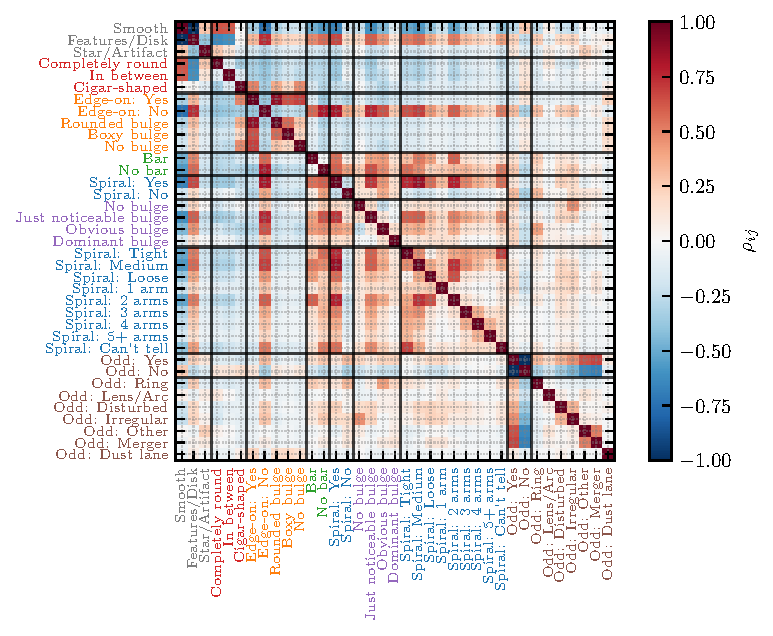
\includegraphics[width=\textwidth]{figures/fig_hierarchical_correlation.pdf}
  \caption{Correlation matrix reordered by tree branch, revealing block structure aligned with the hierarchy.}
  \label{fig:hierarchical_correlation}
\end{figure}

\begin{figure}[H]
  \centering
  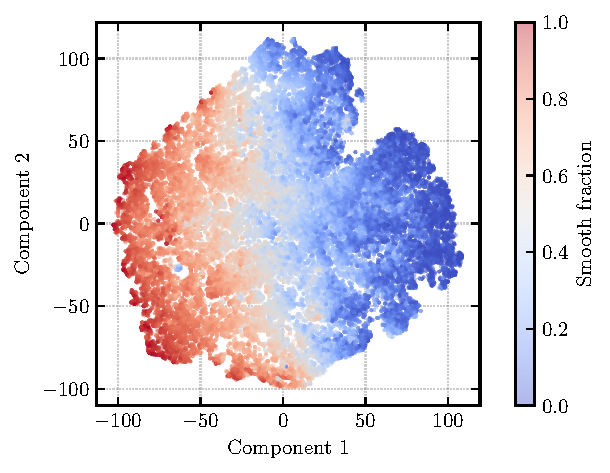
\includegraphics[width=0.7\textwidth]{figures/fig_label_tsne.pdf}
  \caption{t-SNE embedding of the 37-dimensional label space, colored by dominant top-level class.}
  \label{fig:label_tsne}
\end{figure}

\begin{figure}[H]
  \centering
  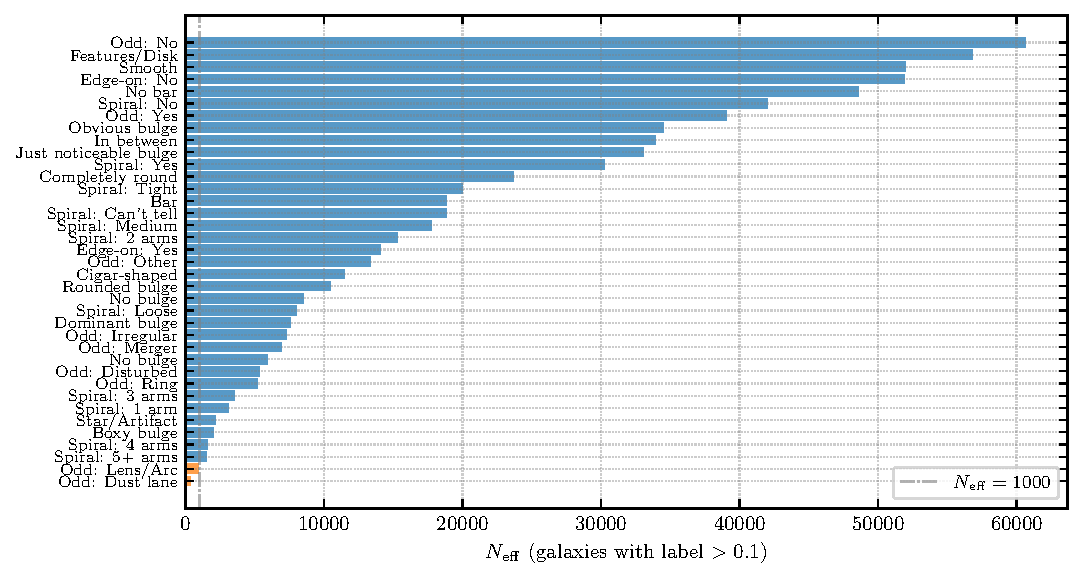
\includegraphics[width=0.8\textwidth]{figures/fig_effective_sample_size.pdf}
  \caption{Effective sample size per label. Hierarchical gating drives deeper-tree labels to $N_{\rm eff}$ far below the nominal 61{,}578.}
  \label{fig:effective_sample_size}
\end{figure}

%%% ---------------------------------------------------------------
\section{Data Preparation}
\label{sec:prep}
%%% ---------------------------------------------------------------

\subsection{Image Downsizing}

Raw SDSS images are $424 \times 424$ pixels, of which most is empty sky. We center-crop (removing 25\% of the border on each side) and resize to $96 \times 96$ pixels, achieving a $\sim$20$\times$ reduction in pixel count while preserving morphological features (Figure~\ref{fig:image_comparison}).

\begin{figure}[H]
  \centering
  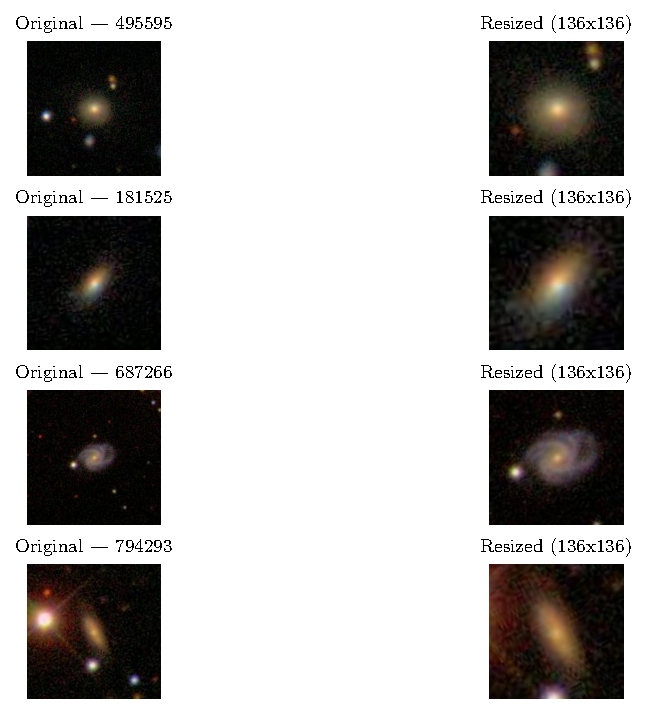
\includegraphics[width=\textwidth]{figures/fig_image_comparison.pdf}
  \caption{Original vs.\ downsized images for four example galaxies.}
  \label{fig:image_comparison}
\end{figure}

\subsection{Train/Validation Split}

We randomly split the dataset 80/20 (seed 42) into 49{,}262 training and 12{,}316 validation images. Figure~\ref{fig:split_distributions} confirms that the label distributions are statistically indistinguishable between the two sets.

\begin{figure}[H]
  \centering
  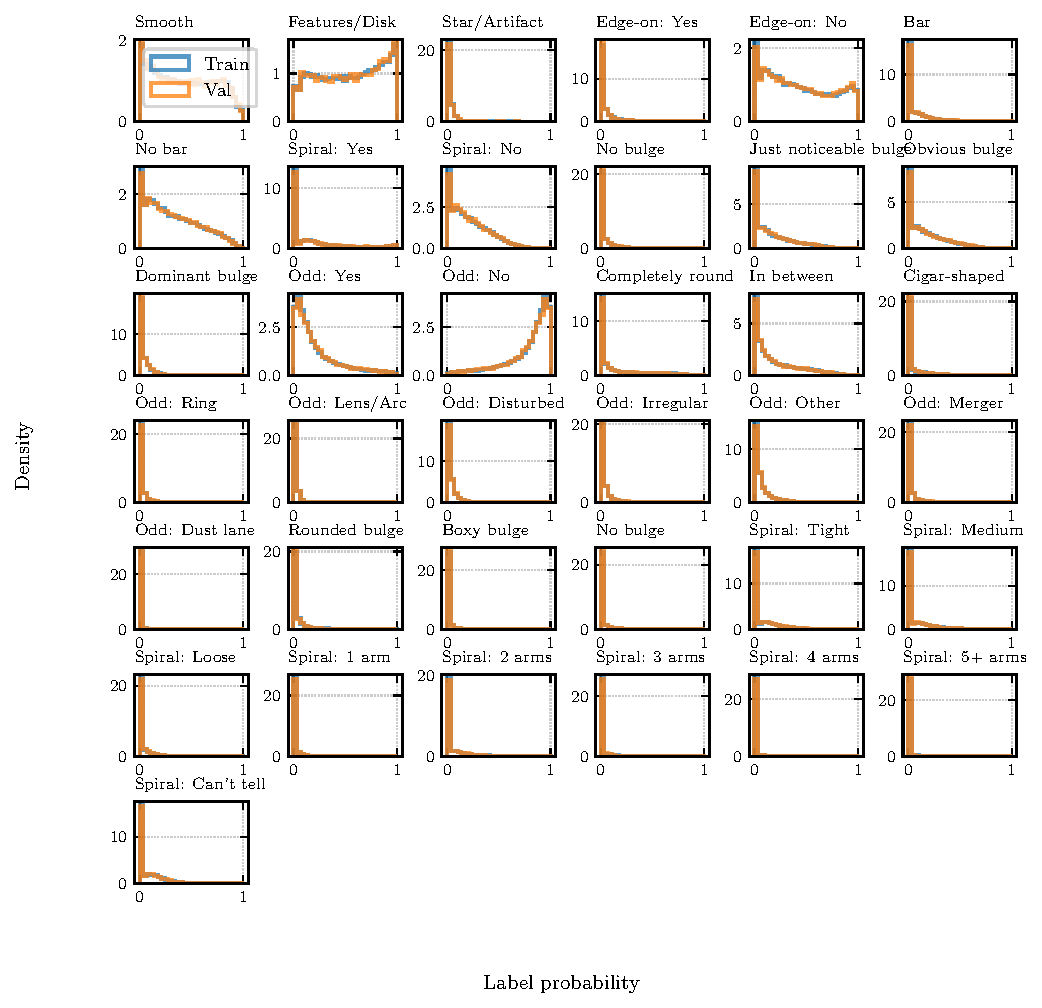
\includegraphics[width=\textwidth]{figures/fig_split_distributions.pdf}
  \caption{Training (blue) vs.\ validation (orange) label distributions.}
  \label{fig:split_distributions}
\end{figure}

\subsection{Baseline Model}

The baseline model predicts the training-set mean label vector for every image, yielding training and validation RMSEs of 0.1638 and 0.1639 respectively. Any CNN must outperform this floor.

%%% ---------------------------------------------------------------
\section{Network Architectures}
\label{sec:architectures}
%%% ---------------------------------------------------------------

We train two backbone architectures: a hand-designed 4-block custom CNN ($\sim$2.8M parameters) and an 18-layer ResNet ($\sim$11.2M parameters). Both consume $96 \times 96 \times 3$ inputs and emit a 37-dimensional sigmoid head; they differ in depth, parameter count, and the use of residual connections. Figure~\ref{fig:architectures} summarizes the layer stacks side-by-side.

\begin{figure*}[t!]
  \centering
  \begin{tikzpicture}[
      layer/.style={circle, draw=black, thick, minimum size=0.7cm,
                    inner sep=0pt, font=\scriptsize},
      input/.style={layer, fill=gray!25},
      conv/.style={layer, fill=blue!20},
      pool/.style={layer, fill=cyan!25},
      res/.style={layer, fill=violet!25},
      fc/.style={layer, fill=orange!25},
      outnode/.style={layer, fill=green!25},
      lbl/.style={font=\scriptsize, align=center},
      conn/.style={-{Stealth[length=4pt]}, thick},
      title/.style={font=\small\bfseries, anchor=east},
      x=1.25cm, y=1cm,
    ]

    % ====== Layout constants ======
    \def\xRaw{-2.0}
    \def\xImg{0}
    \def\xConv{2.3}
    \def\xPool{4.3}
    \def\xFCa{7.9}
    \def\xFCb{9.6}
    \def\xOut{11.5}
    \def\yLbl{-2.05}
    \def\yRes{-5.0}

    % ====== Custom CNN (top row) ======
    % --- Raw full-resolution SDSS image ---
    \node[draw=black, thick, inner sep=1pt] (a_raw)
         at (\xRaw, 0) {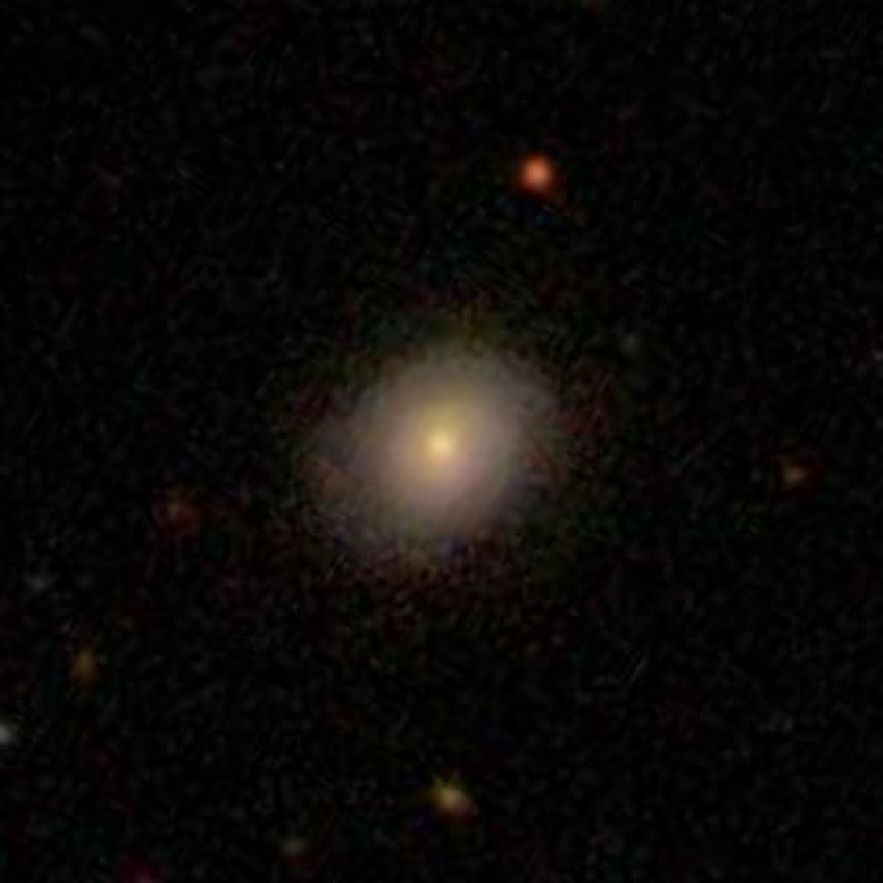
\includegraphics[width=1.5cm]{figures/fig_example_galaxy_full.pdf}};
    \node[lbl] at (\xRaw, \yLbl) {raw SDSS image\\$424{\times}424{\times}3$};

    % --- Resized network input image ---
    \node[draw=black, thick, inner sep=1pt] (a_img)
         at (\xImg, 0) {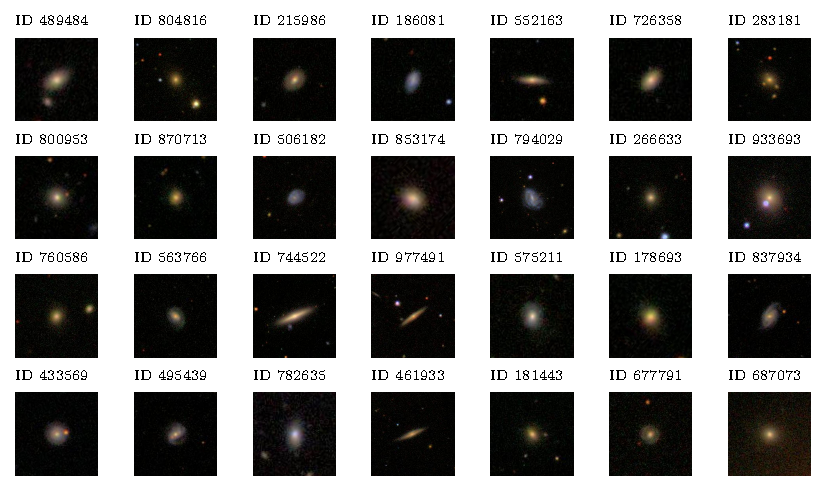
\includegraphics[width=1.2cm]{figures/fig_example_galaxy.pdf}};
    \node[lbl] at (\xImg, \yLbl) {input image\\$96{\times}96{\times}3$};

    % --- Arrow: raw -> resized input ---
    \draw[conn] (a_raw.east) -- (a_img.west);

    % --- Conv stack (3D look) ---
    \begin{scope}[shift={(\xConv, 0)}]
      \foreach \sh in {0,0.09,0.18,0.27} {
        \draw[fill=blue!25, thick]
              (-0.5+\sh, -0.5-\sh) rectangle (0.5+\sh, 0.5-\sh);
      }
    \end{scope}
    \coordinate (a_conv_w) at (\xConv-0.5, 0);
    \coordinate (a_conv_e) at (\xConv+0.77, 0);
    \node[lbl] at (\xConv+0.13, -1.05)
         {Conv $3{\times}3$};

    % --- MaxPool (smaller stack) ---
    \begin{scope}[shift={(\xPool, 0)}]
      \foreach \sh in {0,0.07,0.14,0.21} {
        \draw[fill=cyan!30, thick]
              (-0.3+\sh, -0.3-\sh) rectangle (0.3+\sh, 0.3-\sh);
      }
    \end{scope}
    \coordinate (a_pool_w) at (\xPool-0.3, 0);
    \coordinate (a_pool_e) at (\xPool+0.51, 0);
    \node[lbl] at (\xPool+0.10, -1.05)
         {MaxPool $2{\times}2$};

    % --- Forward arrow inside the block: conv -> pool ---
    \draw[conn] (a_conv_e) -- (a_pool_w);

    % --- Dashed encapsulating box around Conv + MaxPool, labeled ×4 ---
    \node[draw=black, thick, dashed, rounded corners=3pt,
          fit={(\xConv-0.7,0.65) (\xPool+0.75,-1.5)},
          inner sep=0pt,
          label={[font=\scriptsize, align=center, yshift=2pt]above:%
            {Feature extractor block \quad $\times 4$\\
             channels: $32 \to 64 \to 128 \to 256$\\
             resolution: $96 \to 48 \to 24 \to 12 \to 6$}}]
         (a_block) {};

    % --- Image -> block, block -> flatten (forced to y=0 so all aligned) ---
    \coordinate (a_block_w) at (a_block.west |- 0,0);
    \coordinate (a_block_e) at (a_block.east |- 0,0);
    \draw[conn] (a_img.east) -- (a_block_w);
    \coordinate (a_flat) at (\xFCa-0.65, 0);
    \draw[conn] (a_block_e) -- (a_flat)
                node[pos=0.55, above=1pt, font=\scriptsize, align=center]
                  {flatten\\$6{\times}6{\times}256 = 9216$};

    % --- FC layer 1 (3 + vdots + 3 = 6 circles representing 256 units) ---
    \begin{scope}[shift={(\xFCa, 0)}]
      \foreach \i/\y in {0/1.20, 1/0.90, 2/0.60} {
        \node[fc, minimum size=0.34cm, font=\tiny] (f1-\i) at (0, \y) {};
      }
      \node[font=\Large, inner sep=2pt] at (0, 0) {$\vdots$};
      \foreach \i/\y in {3/-0.60, 4/-0.90, 5/-1.20} {
        \node[fc, minimum size=0.34cm, font=\tiny] (f1-\i) at (0, \y) {};
      }
    \end{scope}
    \node[lbl] at (\xFCa, \yLbl) {FC 256};

    % --- FC layer 2 (2 + vdots + 2 = 4 circles representing 128 units) ---
    \begin{scope}[shift={(\xFCb, 0)}]
      \foreach \i/\y in {0/0.90, 1/0.55} {
        \node[fc, minimum size=0.34cm, font=\tiny] (f2-\i) at (0, \y) {};
      }
      \node[font=\Large, inner sep=2pt] at (0, 0) {$\vdots$};
      \foreach \i/\y in {2/-0.55, 3/-0.90} {
        \node[fc, minimum size=0.34cm, font=\tiny] (f2-\i) at (0, \y) {};
      }
    \end{scope}
    \node[lbl] at (\xFCb, \yLbl) {FC 128};

    % --- Output layer (1 + vdots + 1 = 2 circles representing 37 sigmoid units) ---
    \begin{scope}[shift={(\xOut, 0)}]
      \node[outnode, minimum size=0.34cm, font=\tiny] (o-0) at (0, 0.60) {};
      \node[font=\Large, inner sep=2pt] at (0, 0) {$\vdots$};
      \node[outnode, minimum size=0.34cm, font=\tiny] (o-1) at (0, -0.60) {};
    \end{scope}
    \node[lbl] at (\xOut, \yLbl) {37 sigmoid\\outputs};

    % --- Dropout labels above the inter-FC connection bundles ---
    \node[font=\scriptsize, align=center]
      at ({(\xFCa+\xFCb)/2}, 1.55) {dropout 0.5};
    \node[font=\scriptsize, align=center]
      at ({(\xFCb+\xOut)/2}, 1.55) {dropout 0.5};

    % --- Connections between layers ---
    %   flatten -> FC256: full set (no dropout on the flatten input)
    \foreach \i in {0,...,5}
      \draw[gray!55, very thin] (a_flat) -- (f1-\i);
    %   FC256 -> FC128: half edges drawn to depict 50% dropout
    \foreach \i in {0,...,5}
      \foreach \j in {0,...,3} {
        \pgfmathtruncatemacro{\drop}{mod(\i+\j,2)}
        \ifnum\drop=0
          \draw[gray!45, very thin] (f1-\i) -- (f2-\j);
        \fi
      }
    %   FC128 -> output: half edges drawn to depict 50% dropout
    \foreach \j in {0,...,3}
      \foreach \k in {0,1} {
        \pgfmathtruncatemacro{\drop}{mod(\j+\k,2)}
        \ifnum\drop=0
          \draw[gray!45, very thin] (f2-\j) -- (o-\k);
        \fi
      }

    % ====== ResNet-18 (bottom row) ======
    \node[input]   (b0) at (0,    \yRes) {In};
    \node[conv]    (b1) at (1.65, \yRes) {Stem};
    \node[res]     (b2) at (3.3,  \yRes) {S1};
    \node[res]     (b3) at (4.95, \yRes) {S2};
    \node[res]     (b4) at (6.6,  \yRes) {S3};
    \node[res]     (b5) at (8.25, \yRes) {S4};
    \node[pool]    (b6) at (9.9,  \yRes) {GAP};
    \node[outnode] (b7) at (11.5, \yRes) {Out};
    \foreach \i/\j in {b0/b1,b1/b2,b2/b3,b3/b4,b4/b5,b5/b6,b6/b7}
      \draw[conn] (\i) -- (\j);

    \node[lbl, below=0.32cm of b0] {$96^2{\times}3$};
    \node[lbl, below=0.32cm of b1] {Conv $3{\times}3$\\64, stride 1};
    \node[lbl, below=0.32cm of b2] {$2{\times}$BB\\64};
    \node[lbl, below=0.32cm of b3] {$2{\times}$BB\\128, s2};
    \node[lbl, below=0.32cm of b4] {$2{\times}$BB\\256, s2};
    \node[lbl, below=0.32cm of b5] {$2{\times}$BB\\512, s2};
    \node[lbl, below=0.32cm of b6] {global\\avg pool};
    \node[lbl, below=0.32cm of b7] {37,\\sigmoid};

    % --- BasicBlock inset, centered below ResNet ---
    \node[draw=black, thick, dashed, rounded corners=3pt,
          font=\scriptsize, align=center, inner sep=6pt,
          anchor=north] (bb) at (5.75, \yRes-1.5) {%
      \textbf{BasicBlock (BB)}\\[3pt]
      \begin{tikzpicture}[
          baseline, x=0.9cm,
          mini/.style={circle, draw=black, thick, minimum size=0.5cm,
                       inner sep=0pt, font=\tiny, fill=blue!20},
          sumn/.style={circle, draw=black, thick, minimum size=0.42cm,
                       inner sep=0pt, font=\tiny, fill=white},
          mconn/.style={-{Stealth[length=3pt]}, thick},
        ]
        \node[mini] (m1) at (0,0)   {C};
        \node[mini] (m2) at (1.2,0) {C};
        \node[sumn] (ms) at (2.4,0) {$+$};
        \node[mini, fill=green!25] (mr) at (3.6,0) {R};
        \draw[mconn] (m1) -- (m2);
        \draw[mconn] (m2) -- (ms);
        \draw[mconn] (ms) -- (mr);
        \draw[mconn] (m1) to[bend left=55] (ms);
        \node[font=\tiny] at (1.2, 0.6) {skip};
      \end{tikzpicture}
    };
  \end{tikzpicture}
  \caption{Architecture flow for the two backbones, read left-to-right. \emph{Top --- Custom CNN ($\sim$2.8M params):} a $96\times96\times3$ input image passes through a convolutional feature extractor consisting of a stack of $3\times3$ convolutions followed by $2\times2$ max-pooling, with the dashed loop indicating the block is repeated four times at channel widths $32 \to 64 \to 128 \to 256$. The flattened feature vector is then fully connected to 256 units, halved to 128 units, and finally projected onto 37 sigmoid outputs. Edges between FC layers are drawn schematically. \emph{Bottom --- ResNet-18 ($\sim$11.2M params):} a $3\times3$/stride-1 stem (no initial max-pool, suitable for the small $96\times96$ input) feeds four residual stages (S1--S4) of two BasicBlocks each at channel widths 64/128/256/512, ending in global average pooling and a 37-way sigmoid head. The dashed inset shows the internal flow of one BasicBlock: two $3\times3$ convolutions (C) summed with the identity skip ($+$) followed by ReLU (R).}
  \label{fig:architectures}
\end{figure*}

%%% ---------------------------------------------------------------
\section{ResNet-18}
\label{sec:resnet}
%%% ---------------------------------------------------------------

Residual Networks \citep{He2015} address the degradation problem in deep CNNs via skip connections that add the block input directly to its output: $H(x) = F(x) + x$. We use an 18-layer ResNet modified for our $96 \times 96$ input (3$\times$3 first conv, stride 1, no initial max-pool) and a 37-output sigmoid head. The plain model (50 epochs, Adam) attains a validation RMSE of 0.1004. Figure~\ref{fig:loss_resnet_18} shows the training and validation loss curves.

\begin{figure}[H]
  \centering
  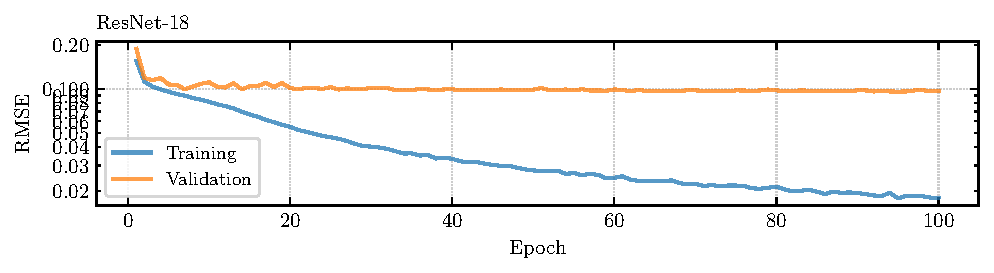
\includegraphics[width=0.5\textwidth]{figures/fig_loss_resnet_18.pdf}
  \caption{ResNet-18 training and validation RMSE vs.\ epoch.}
  \label{fig:loss_resnet_18}
\end{figure}

%%% ---------------------------------------------------------------
\section{Custom CNN}
\label{sec:custom}
%%% ---------------------------------------------------------------

Our custom CNN uses four convolutional blocks (32, 64, 128, 256 channels, each with $3\times3$ kernels, ReLU, and max pooling) followed by two fully connected layers (256, 128 units) with 50\% dropout and a 37-way sigmoid output. The architecture has $\sim$2.8M parameters, roughly a quarter of ResNet-18's $\sim$11.2M, and reaches a validation RMSE of 0.0985. Figure~\ref{fig:loss_custom_cnn} shows the loss curves.

\begin{figure}[H]
  \centering
  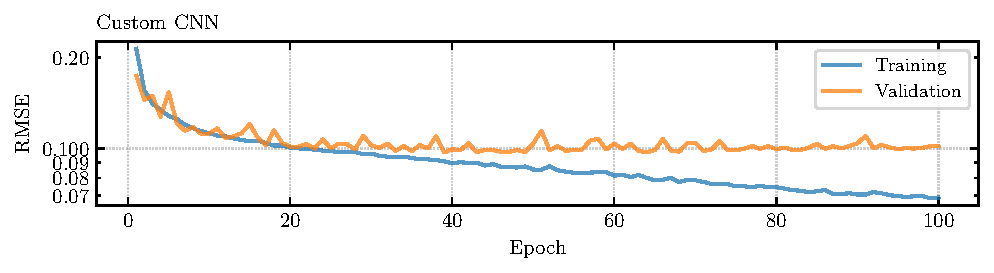
\includegraphics[width=0.5\textwidth]{figures/fig_loss_custom_cnn.pdf}
  \caption{Custom CNN training and validation RMSE vs.\ epoch.}
  \label{fig:loss_custom_cnn}
\end{figure}

%%% ---------------------------------------------------------------
\section{Optimization}
\label{sec:opt}
%%% ---------------------------------------------------------------

\subsection{Learning Rate Scheduling}

We retrain both backbones with \texttt{ReduceLROnPlateau} (factor 0.5, patience 3 epochs), which decreases the learning rate whenever the validation loss plateaus and enables finer convergence. Figures~\ref{fig:loss_lr_resnet} and \ref{fig:loss_lr_custom} show the resulting loss and learning-rate trajectories for the ResNet-18 and the custom CNN respectively. The scheduler reduces the validation RMSE of the ResNet to 0.0977 and of the custom CNN to a comparable value.

\begin{figure}[H]
  \centering
  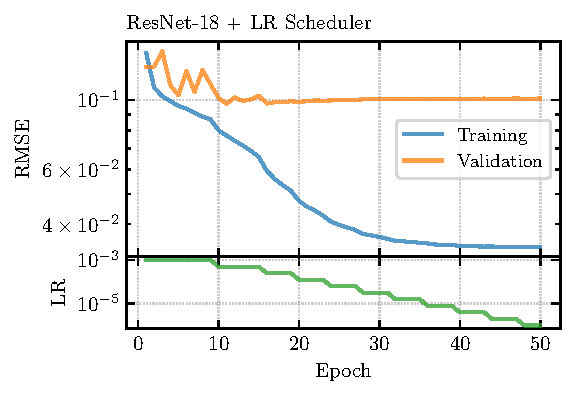
\includegraphics[width=0.5\textwidth]{figures/fig_loss_lr_resnet_18_+_lr_scheduler.pdf}
  \caption{ResNet-18 with LR scheduler: loss curves (top) and learning rate (bottom).}
  \label{fig:loss_lr_resnet}
\end{figure}

\begin{figure}[H]
  \centering
  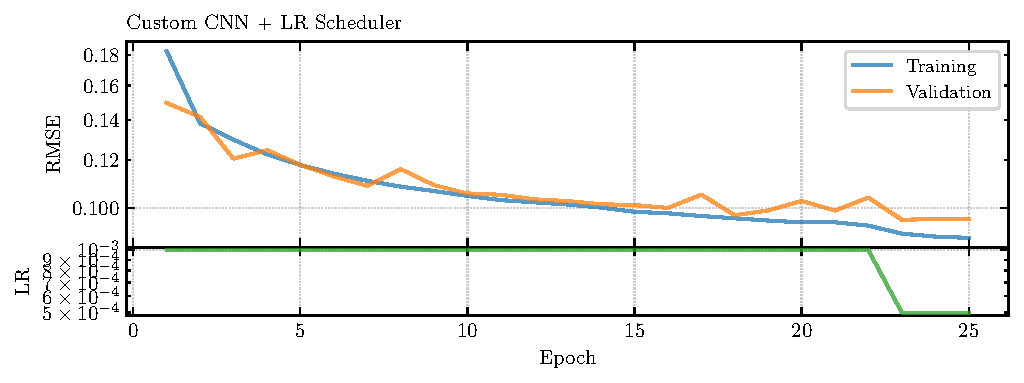
\includegraphics[width=0.5\textwidth]{figures/fig_loss_lr_custom_cnn_+_lr_scheduler.pdf}
  \caption{Custom CNN with LR scheduler: loss curves (top) and learning rate (bottom).}
  \label{fig:loss_lr_custom}
\end{figure}

\subsection{Data Augmentation}

Galaxy morphological labels are rotationally invariant: a spiral galaxy remains a spiral under arbitrary rotation. We augment the training set by rotating each image by a uniformly random angle $\theta \in [0, 360)$ degrees, combined with the LR scheduler. Figures~\ref{fig:loss_lr_aug_resnet} and \ref{fig:loss_lr_aug_custom} show the improved loss curves with reduced overfitting for both backbones. The augmented ResNet attains the best overall validation RMSE of 0.0965.

\begin{figure}[H]
  \centering
  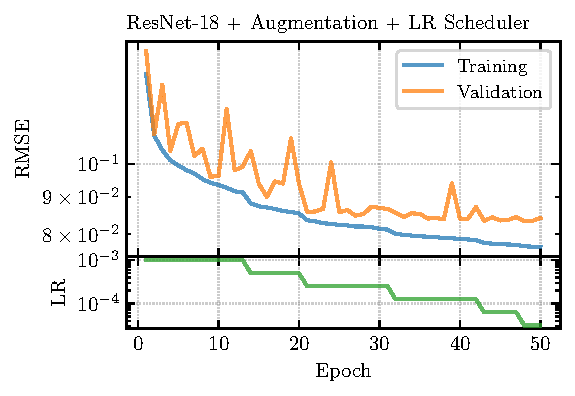
\includegraphics[width=0.5\textwidth]{figures/fig_loss_lr_resnet_18_+_augmentation_+_lr_scheduler.pdf}
  \caption{ResNet-18 with augmentation + LR scheduler.}
  \label{fig:loss_lr_aug_resnet}
\end{figure}

\begin{figure}[H]
  \centering
  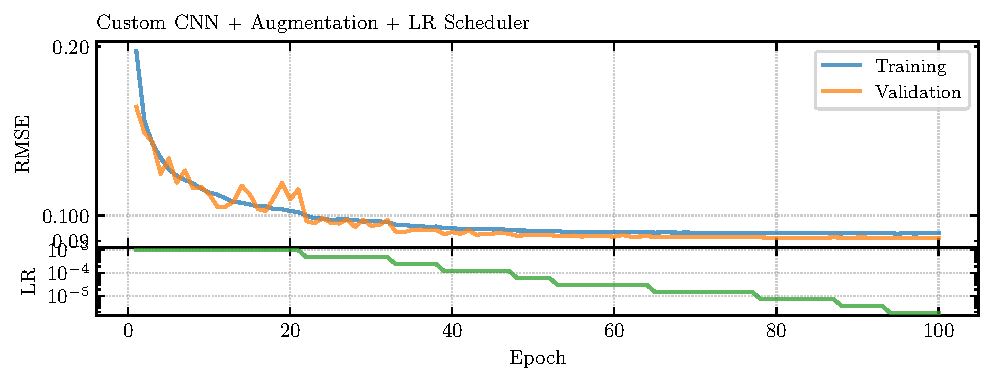
\includegraphics[width=0.5\textwidth]{figures/fig_loss_lr_custom_cnn_+_augmentation_+_lr_scheduler.pdf}
  \caption{Custom CNN with augmentation + LR scheduler.}
  \label{fig:loss_lr_aug_custom}
\end{figure}

%%% ---------------------------------------------------------------
\section{Model Comparison and Evaluation}
\label{sec:eval}
%%% ---------------------------------------------------------------

\subsection{Model Comparison}

Figure~\ref{fig:model_comparison} compares validation RMSE across all trained models. Table~\ref{tab:model_rmse} summarizes the best validation RMSE for each. The ResNet-18 with augmentation and LR scheduling achieves the best performance, a $\sim$41\% reduction below the mean-prediction baseline.

\begin{table}[H]
  \centering
  \begin{tabular}{lc}
    \toprule
    Model & Best Val.\ RMSE \\
    \midrule
    Mean-prediction baseline & 0.1639 \\
    ResNet-18 (plain) & 0.1004 \\
    Custom CNN (plain) & 0.0985 \\
    ResNet-18 + LR scheduler & 0.0977 \\
    ResNet-18 + augmentation + LR scheduler & \textbf{0.0965} \\
    \bottomrule
  \end{tabular}
  \caption{Best validation RMSE achieved by each model.}
  \label{tab:model_rmse}
\end{table}

\begin{figure}[H]
  \centering
  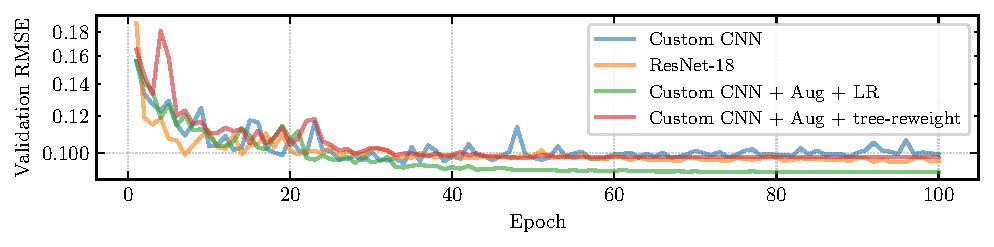
\includegraphics[width=0.5\textwidth]{figures/fig_model_comparison.pdf}
  \caption{Validation RMSE comparison across three models.}
  \label{fig:model_comparison}
\end{figure}

\subsection{Per-Label Performance}

Figure~\ref{fig:label_scatter} shows true vs.\ predicted scatter plots for all 37 labels on the validation set using the best model. Top-level features (smooth, disk) track the 1:1 line well; rare features (merger, ring, lens/arc) show larger scatter and regression toward the mean, reflecting the sparse training signal.

\begin{figure}[H]
  \centering
  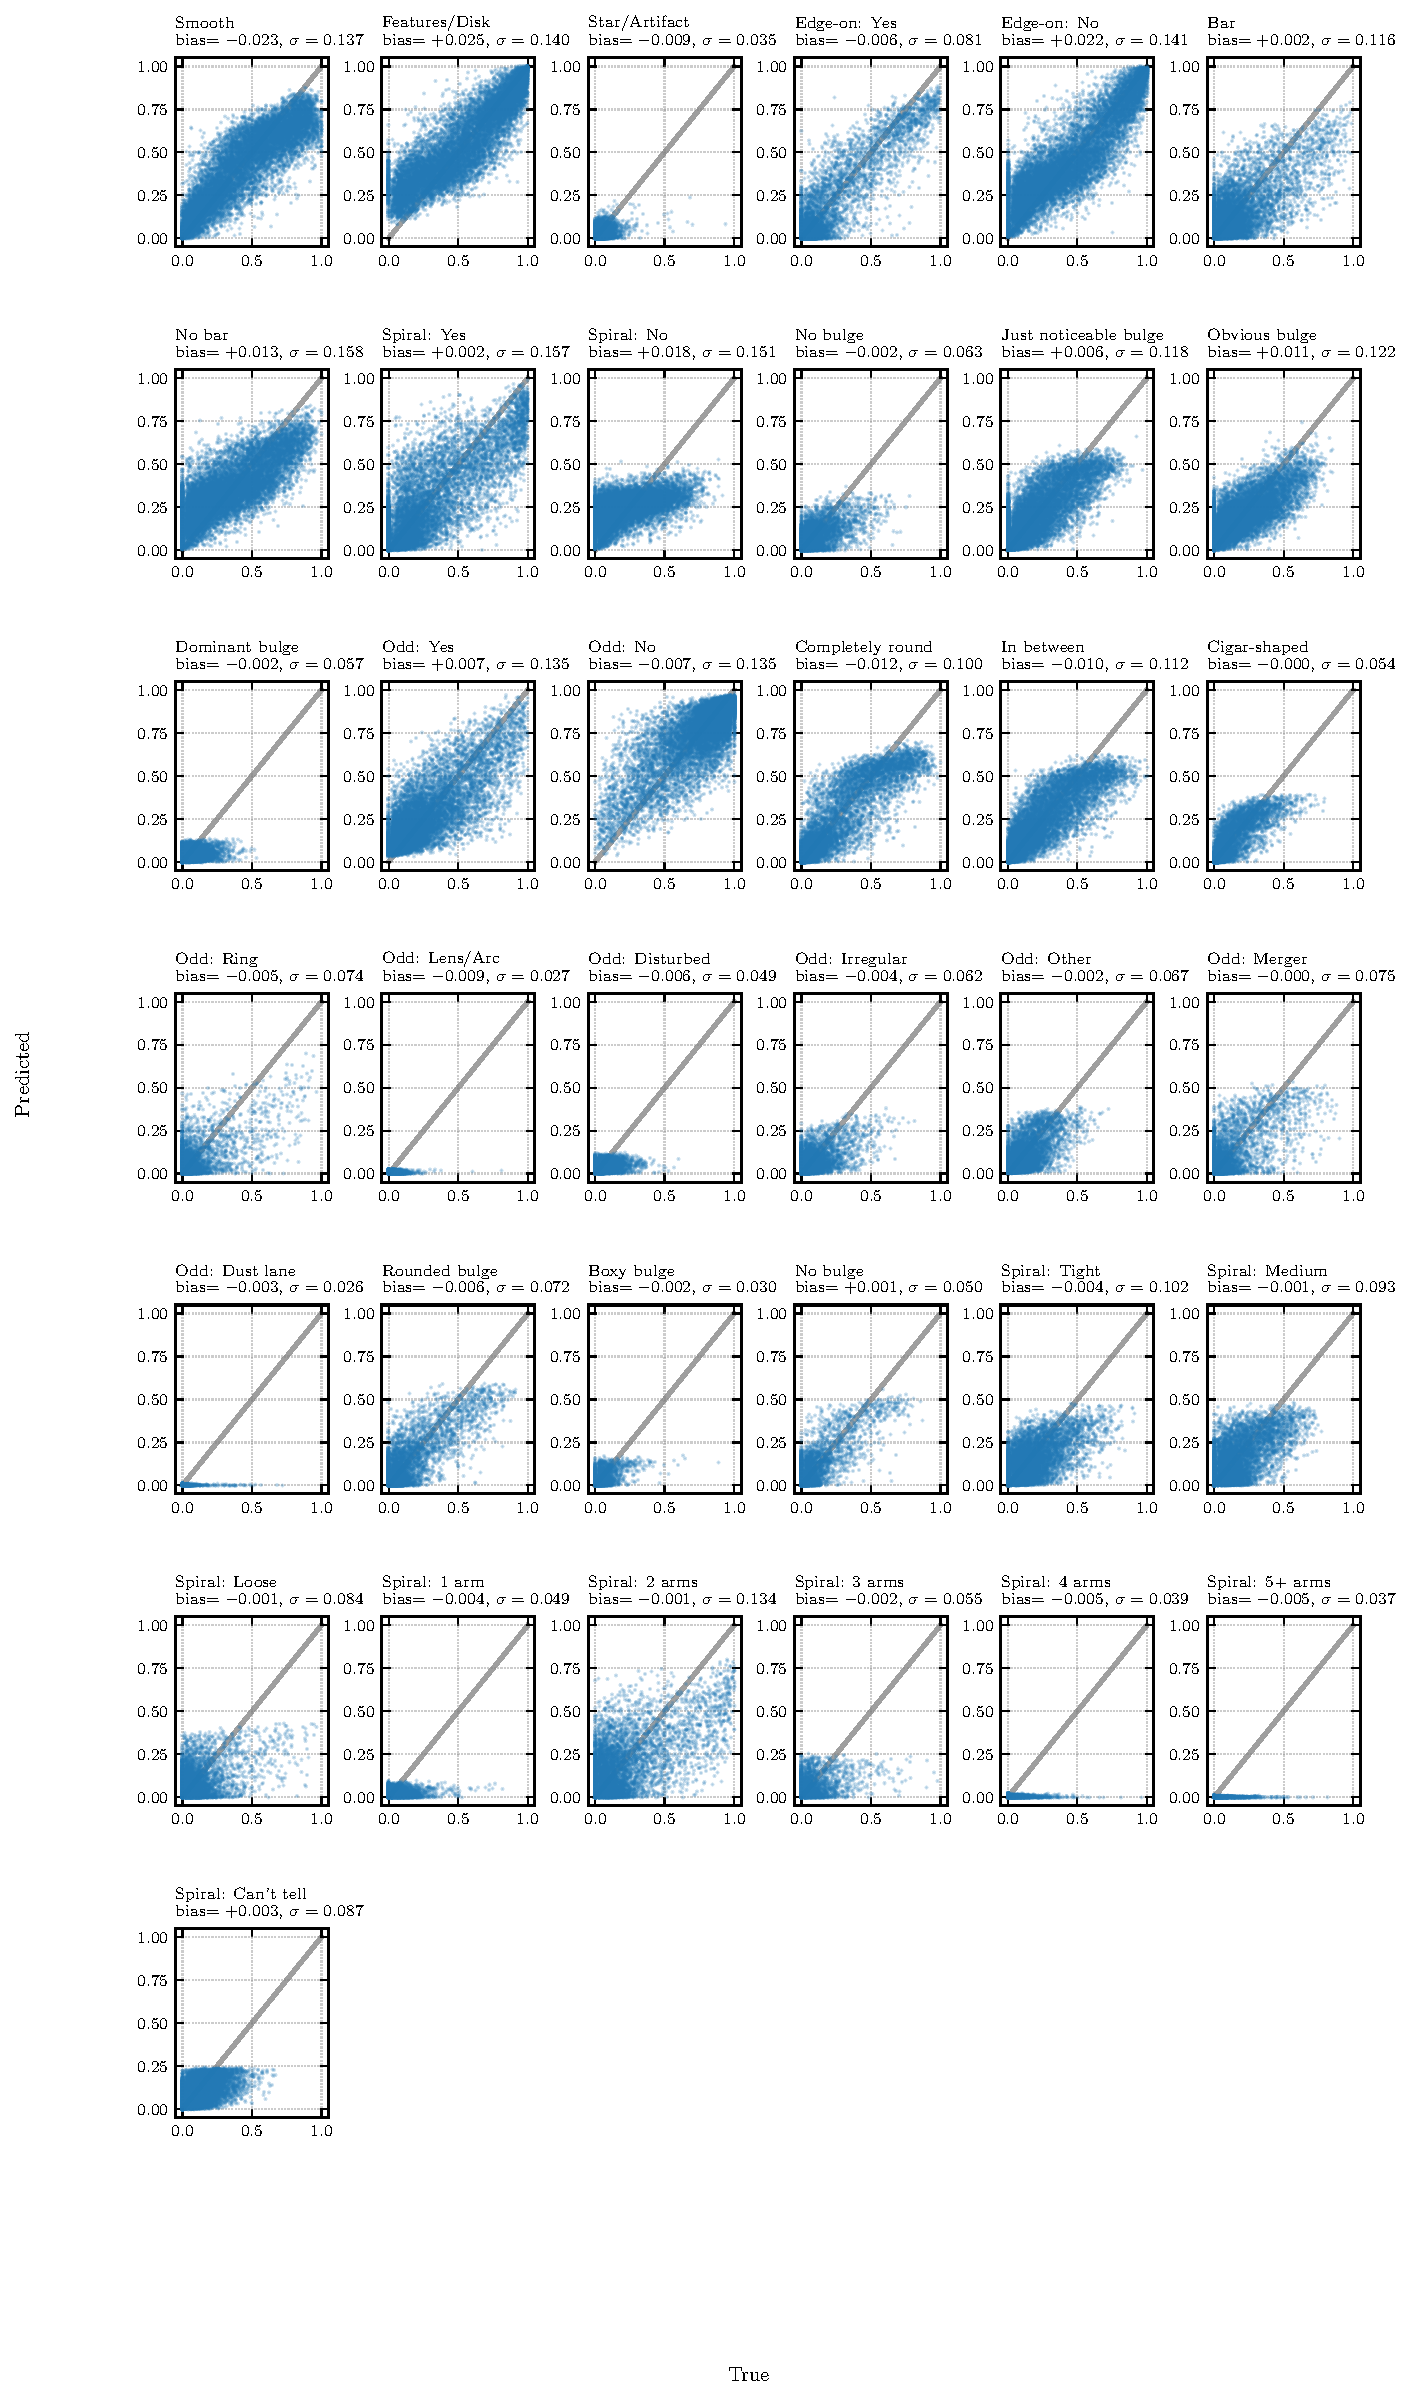
\includegraphics[width=\textwidth]{figures/fig_label_scatter.pdf}
  \caption{True vs.\ predicted label values for all 37 labels (validation set). Diagonal line is 1:1; bias and scatter annotated per panel.}
  \label{fig:label_scatter}
\end{figure}

\subsection{Extreme Examples}

Figures~\ref{fig:top5_smooth}--\ref{fig:top5_odd_merger} show the top-5 most extreme validation images for 7 labels, comparing actual (top row) vs.\ predicted (bottom row) rankings.

\begin{figure}[H]
  \centering
  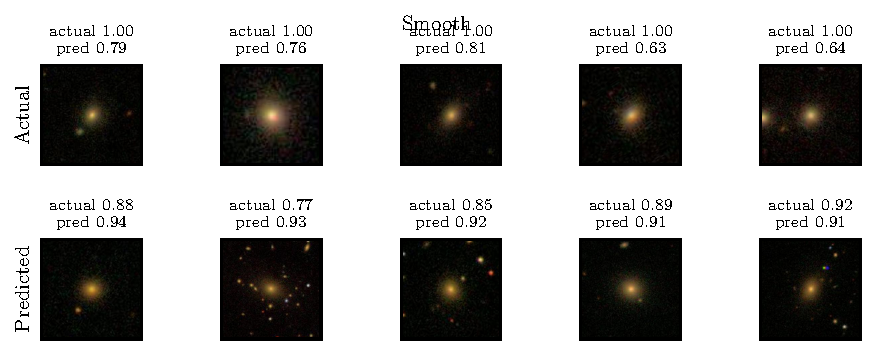
\includegraphics[width=0.8\textwidth]{figures/fig_top5_smooth.pdf}
  \caption{Top-5 images for ``Smooth'' by actual (top) and predicted (bottom) label.}
  \label{fig:top5_smooth}
\end{figure}

\begin{figure}[H]
  \centering
  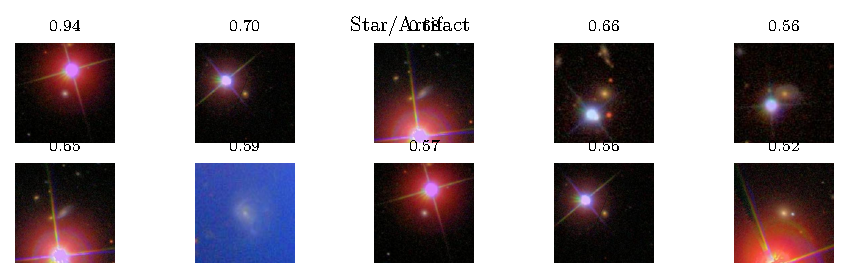
\includegraphics[width=0.8\textwidth]{figures/fig_top5_star_artifact.pdf}
  \caption{Top-5 images for ``Star/Artifact.''}
  \label{fig:top5_star}
\end{figure}

\begin{figure}[H]
  \centering
  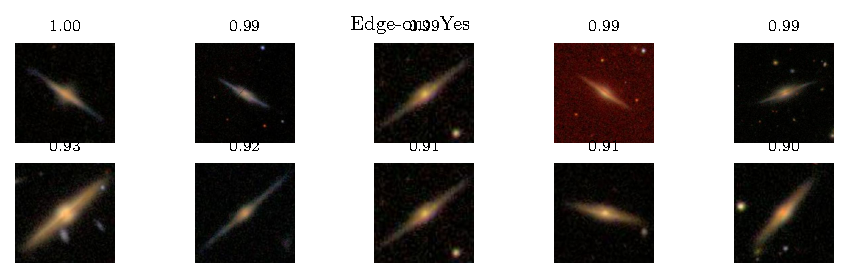
\includegraphics[width=0.8\textwidth]{figures/fig_top5_edge-on_yes.pdf}
  \caption{Top-5 images for ``Edge-on: Yes.''}
  \label{fig:top5_edgeon}
\end{figure}

\begin{figure}[H]
  \centering
  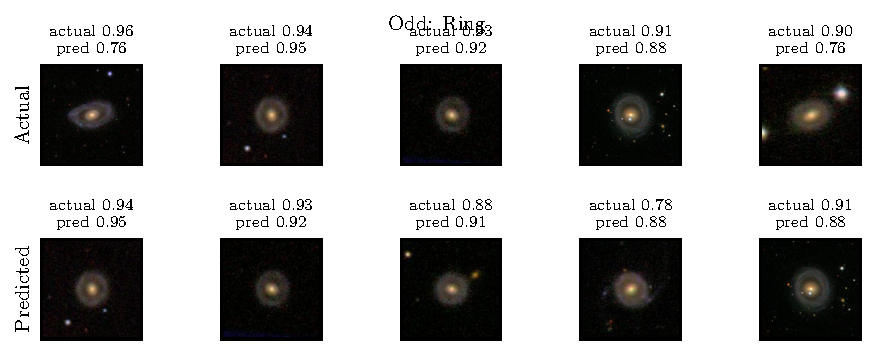
\includegraphics[width=0.8\textwidth]{figures/fig_top5_odd_ring.pdf}
  \caption{Top-5 images for ``Odd: Ring.''}
  \label{fig:top5_ring}
\end{figure}

\begin{figure}[H]
  \centering
  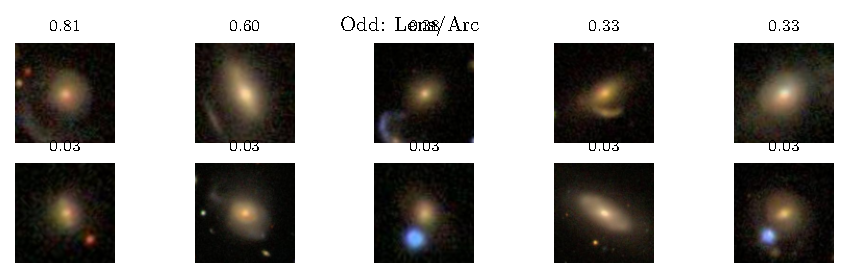
\includegraphics[width=0.8\textwidth]{figures/fig_top5_odd_lens_arc.pdf}
  \caption{Top-5 images for ``Odd: Lens/Arc.''}
  \label{fig:top5_lens}
\end{figure}

\begin{figure}[H]
  \centering
  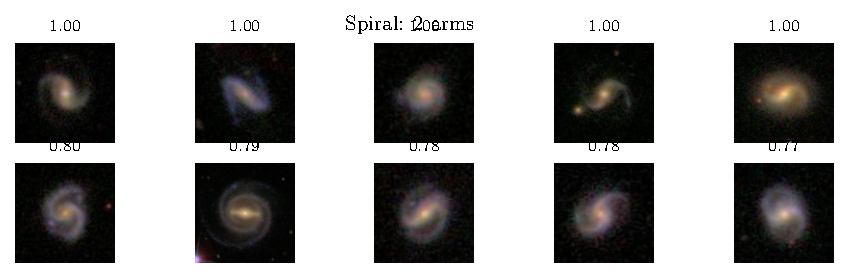
\includegraphics[width=0.8\textwidth]{figures/fig_top5_spiral_2_arms.pdf}
  \caption{Top-5 images for ``Spiral: 2 arms.''}
  \label{fig:top5_spiral}
\end{figure}

\begin{figure}[H]
  \centering
  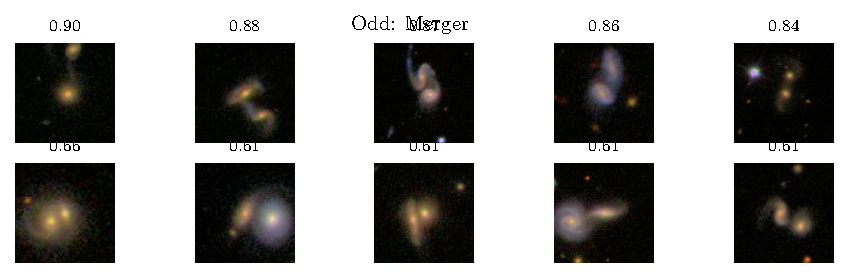
\includegraphics[width=0.8\textwidth]{figures/fig_top5_odd_merger.pdf}
  \caption{Top-5 images for ``Odd: Merger.''}
  \label{fig:top5_merger}
\end{figure}

%%% ---------------------------------------------------------------
\section{Merger Fraction}
\label{sec:mergers}
%%% ---------------------------------------------------------------

We apply the best-performing model (augmented ResNet-18 with LR scheduling) to a held-out set of 79{,}975 test images and estimate the galaxy merger fraction as the mean predicted probability of the ``Odd: Merger'' label (Class8.6). We obtain a merger fraction of $\sim$4.3\%. The Lotz et al.\ (2011) $z \approx 0$ major merger rate is $\sim$0.01--0.03~Gyr$^{-1}$; converting to an instantaneous merger fraction requires multiplying by the merger observability timescale $T_{\rm obs} \sim 0.5$--1~Gyr, giving an expected fraction of $\sim$0.5--3\%, modestly below our estimate.

Several factors complicate direct comparison: (1)~the GZ2 ``merger'' label conflates major and minor mergers, tidal interactions, and close pairs; (2)~higher-redshift galaxies appear smaller and may be preferentially classified as disturbed; (3)~the Lotz et al.\ rates are in units of Gyr$^{-1}$ (a rate), while we estimate a dimensionless fraction; (4)~GZ2 debiasing corrections do not fully account for resolution-dependent classification bias.

%%% ---------------------------------------------------------------
\section{Conclusion}
\label{sec:conclusion}
%%% ---------------------------------------------------------------

We have demonstrated that CNNs can predict Galaxy Zoo 2 morphological labels from SDSS images with RMSE well below the mean-prediction baseline. Data augmentation via random rotation and learning rate scheduling provide substantial improvements, exploiting the rotational invariance of galaxy morphology. The trained model enables automated estimation of the galaxy merger fraction on large image sets, although careful interpretation is required to compare with theoretical merger rates due to differences in definition and timescale.

\bibliography{references}
\bibliographystyle{aasjournal}

\end{document}
